The purpose of this section is to answer both the checkpoint and report
questions of the HTTP lab sessions, as well as discuss any relevant results
obtained during the experiences.

\subsection{HTTP GET/response}
After starting Wireshark and choosing a network device, several live packets
are displayed, along with their source and destination IPs, the protocol used,
length, and summarized information. For this experience, we applied a filter to
focus only on HTTP messages.

After visiting the requested url on our browser, two packets were immediately
displayed.

\begin{figure}[htbp]
    \centering
    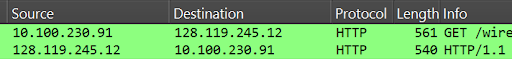
\includegraphics[width=1\linewidth]{img/1.png}
    \caption{Captured packets}\label{fig:1}
\end{figure}

Clicking a packet reveals a window on the lower side of the screen, which
displays the information contained in the HTTP message. At a glance, we can see
that our browser used HTTP 1.1 for its request. This is probably due to the url
using \textit{HTTP} instead of \textit{HTTPS}.

\begin{figure}[htbp]
    \centering
    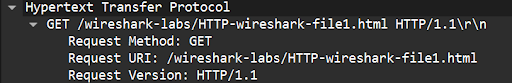
\includegraphics[width=1\linewidth]{img/2.png}
    \caption{HTTP version (request)}\label{fig:2}
\end{figure}

Similarly, clicking the response packet displays that the same HTTP version was
used by the server when sending its response.

\begin{figure}[htbp]
    \centering
    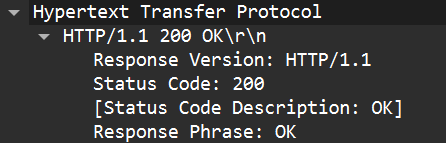
\includegraphics[width=1\linewidth]{img/3.png}
    \caption{HTTP version (response)}\label{fig:3}
\end{figure}

After checking the HTTP versions, we can find both source and destination IPs,
i.e our computer and the server, on the top viewport of the screen, as shown in
Figure~\ref{fig:1}. Our IP is 10.100.230.91, and the IP corresponding to
gaia.cs.umass.edu is 128.119.245.12.\\

The status code returned from the server is 200, as displayed in
Figure~\ref{fig:3}.\\

After checking the section just below the information display in Figure 3, we
can see that the requested HTML file was last modified at 27/08, 5:59.01, GMT
time zone. This is just moments before the time of request, which makes sense
as the server is configured to change the HTML file's modification time each
minute.

\begin{figure}[htbp]
    \centering
    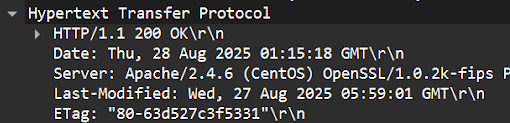
\includegraphics[width=1\linewidth]{img/4.png}
    \caption{Last-Modified}\label{fig:4}
\end{figure}

In a different section, we can see that the length of the response is 526
bytes, while the HTML file itself accounts for 128 bytes of the total length.

\begin{figure}[htbp]
    \centering
    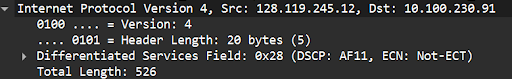
\includegraphics[width=1\linewidth]{img/5.png}
    \caption{Response length}\label{fig:5}
\end{figure}

\begin{figure}[htbp]
    \centering
    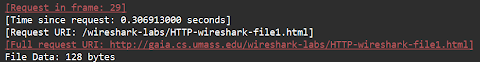
\includegraphics[width=1\linewidth]{img/6.png}
    \caption{HTML length}\label{fig:6}
\end{figure}

In the lower viewport, that is, the packet listing window, we can see the
headers used by both requests and responses. Alternatively, this information
can also be seen in the raw data window, so we can conclude that Wireshark
shows all of the available information in the raw data section.

\subsection{HTTP conditional GET/response}
After inspecting the contents of the first HTTP GET request, we can see that
the If-Modified-Since header is not present in this packet.

\begin{figure}[htbp]
    \centering
    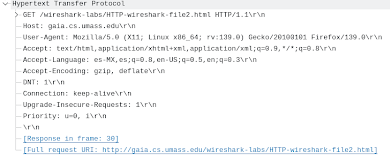
\includegraphics[width=1\linewidth]{img/7.png}
    \caption{If-Modified-Since check}\label{fig:7}
\end{figure}

Looking at the server response, the Content Type or File Data fields are not
present, so the server didn't explicitly return the contents of the file.

\begin{figure}[htbp]
    \centering
    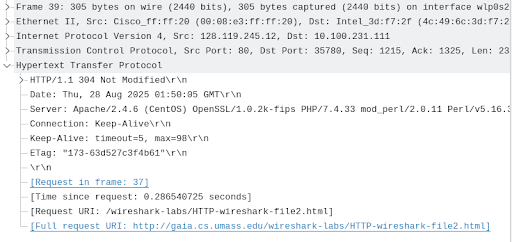
\includegraphics[width=1\linewidth]{img/8.png}
    \caption{Server response}\label{fig:8}
\end{figure}

Inspecting the contents of the second HTTP GET request reveals the
If-Modified-Since header, followed by the timestamp Wed, 27 Aug 2025 05:59:01
GMT.\@

\begin{figure}[htbp]
    \centering
    
\includegraphics[width=1\linewidth]{img/9.png}
    \caption{If-Modified-Since timestamp}\label{fig:9}
\end{figure}

The server's response to the second HTTP GET request was ''304, Not Modified'',
which suggests that since the file was not modified in the server since the
specified timestamp, the server did not return the contents of the file.
Instead, the browser loaded its cached version.

\begin{figure}[htbp]
    \centering
    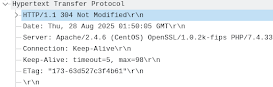
\includegraphics[width=1\linewidth]{img/10.png}
    \caption{304 Not Modified}\label{fig:10}
\end{figure}

\subsection{Retrieving long documents}
During this section of the lab experience, we experimented with larger HTML
files. Data is transmitted in fixed-size segments, so if a file is large
enough, it will be split and transmitted as separate parts.

Even when the requested file is quite large, the browsers sends a single GET
request, and the response is similar to previous request (200, OK). These
results are shown in the next two figures.

\begin{figure}[htbp]
    \centering
    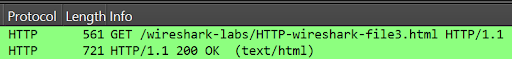
\includegraphics[width=1\linewidth]{img/11.png}
    \caption{HTTP GET for large file}\label{fig:11}
\end{figure}

\begin{figure}[htbp]
    \centering
    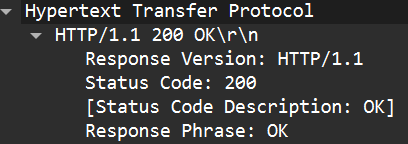
\includegraphics[width=1\linewidth]{img/12.png}
    \caption{HTTP Response}\label{fig:12}
\end{figure}

The HTTP response and HTML file had to be divided in 4 TCP segments, as the
total packet length is 4861 bytes. The HTML accounts for 4500 bytes of the
total length.

\begin{figure}[htbp]
    \centering
    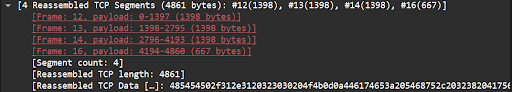
\includegraphics[width=1\linewidth]{img/13.png}
    \caption{TCP Segments}\label{fig:13}
\end{figure}

\subsection{HTML documents with embedded objects}
This lab experience's goal is to understand what happens when a browser
downloads an HTML file with embedded objects, such as images or videos. As
these resources are usually stored in other servers, extra GET requests are
needed.

After visiting the required webpage, which consisted of some plain text and two
images.The IP addresses are displayed as well, and the destination addresses
for the resources are different as they are hosted on different services. The
packets are displayed on the following figure.

\begin{figure}[htbp]
    \centering
    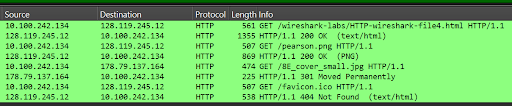
\includegraphics[width=1\linewidth]{img/14.png}
    \caption{Embedded objects GET requests}\label{fig:14}
\end{figure}

Correctly identifying whether the browser downloaded the files serially or in
parallel was a slightly harder task. There is no explicit indicator of this in
the HTTP data window, the requests arrival times were analyzed.

\begin{figure}[htbp]
    \centering
    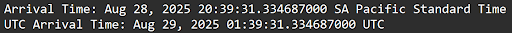
\includegraphics[width=1\linewidth]{img/15.png}
    \caption{PNG image arrival time}\label{fig:15}
\end{figure}

\begin{figure}[htbp]
    \centering
    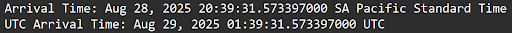
\includegraphics[width=1\linewidth]{img/16.png}
    \caption{JPEG image arrival time}\label{fig:16}
\end{figure}

As both are slightly different, and this situation also occurs with the
responses arrival times, we can conclude that the images were downloaded
serially.

\subsection{HTTP authentication}
This section of the report aims to show the development of the 5th checkpoint,
which focuses mainly on HTTP authentication.

The initial server's response was (401, Unauthorized). However, inputting the
correct credentials allowed us to see the webpage content, and it also added a
new ``Authorization'' field to the HTTP request. Its content consists of the
word ``Basic'' followed by what we considered mostly gibberish, but after
inserting the data into a base64 decoder, we realized that it was actually the
credentials we had inputted earlier.

\begin{figure}[htbp]
    \centering
    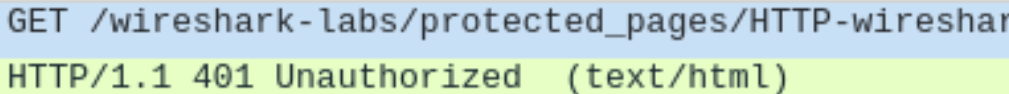
\includegraphics[width=1\linewidth]{img/17.png}
    \caption{Initial Unauthorized response}\label{fig:17}
\end{figure}

\begin{figure}[htbp]
    \centering
    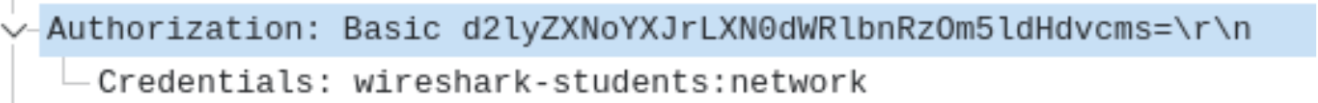
\includegraphics[width=1\linewidth]{img/18.png}
    \caption{Authorization field content}\label{fig:18}
\end{figure}

\begin{figure}[htbp]
    \centering
    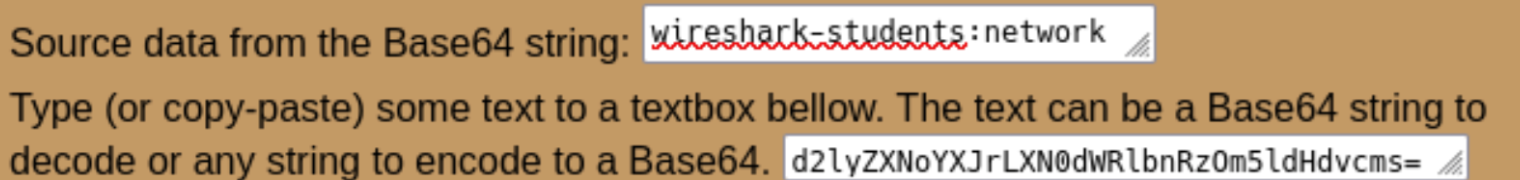
\includegraphics[width=1\linewidth]{img/19.png}
    \caption{Decoded base64 credentials}\label{fig:19}
\end{figure}